
\section{Two Neuron Connections}

Connectivity in cortical neural networks shows a specific . First
described by Markram 1997, finding across have confirmed . 

A first result

In anisotropic networks an overrepresentation of reciprocal
connections is present. Counting and comparing it with our expectation
from Gilbert random graphs $G(n,p)$, In random graphs the probabilities
that a random pair of vertices are 

\begin{align*}
Pr[\abs{}\mathrm{unconnected}] & = (1-p)^2, \\
& = 2 p (1-p) \quad \mathrm{and}\\
& = p^2 \\
\end{align*}
 


\begin{figure}[htp]
  \centering
  \makebox{%
    \begin{overpic}[height=0.17\textheight]{%
        plots/c5f1462b_aniso_rand.pdf}
      \put(13.1,64.8){\small\textbf{A}}
      %\put(14.3,78.9){\small\textbf{A}}
    \end{overpic}
    \hspace{0.45cm}
    \begin{overpic}[height=0.17\textheight]{%
        plots/c5f1462b_aniso_rew.pdf}      
      \put(15.8,64.8){\small\textbf{B}}
    \end{overpic}
  }%
  \vspace{0.2cm}
  \caption{\textbf{Overrepresentation of reciprocal connections in
      anisotropic networks due to distance-dependent connectivity}
    Extracting the counts of unconnected, one-directionally and
    bidirectionally connected neuron pairs in the anisotropic sample
    graphs, overrepresentation of reciprocally connected pairs is
    identified as a feature of the network's distance dependency as
    opposed to anisotropy in connectivity. \textbf{A)} Showing the
    quotient of the counts for the three pair types, extracted from the
    set of sample graphs, with the number of expected pairs in Gilbert
    random graphs $G(n,p)$, where $n=1000$ and $p=0.116$ were matched
    to the sample graph parameters. While single connections appear
    less often than in Gilbert random graphs, reciprocal connections
    are significantly overrepresented. Errorbars SEM. \textbf{B)}
    Comparing appearance of connection pairs in the anisotropic sample
    graphs with their respective appearance in the rewired sample
    graphs, we find that eliminating anisotropy does not significantly
    change the counts for the connection types, indicating that
    anisotropy does not influence two neuron connection
    probabilities. Errorbars SEM.  (\smtcite{c5f1462b})}
  \label{fig:two_neuron_probs}
\end{figure}  

We can further support our hypothesis that anisotropy does not
influence two neuro connection probabilities by calculating them
. Taking distance-dependent connection probability $C(x)$ in
anisotropic networks from Theorem ?? and the , we find the expressions

\begin{align*}
Pr[\abs{}\mathrm{unconnected}] & = \int_0^{\sqrt{2}} (1-C(x))^2 f(x)\,
dx, \\
& = \int_0^{\sqrt{2}} 2 C(x) (1-C(x)) f(x) \, dx \quad \mathrm{and}\\
& = \int_0^{\sqrt{2}} C(x)^2 f(x) \, dx \\
\end{align*}

% From Python c5f1462b
% Unconn:       0.790732332332  +- 0.000817274958369
% Single:       0.184638238238  +- 0.00074516663005
% Recip:        0.0246294294294  +- 8.63947164473e-05


% Mathematica (expected_two_neuron.nb)
% Unconn:       0.791336
% Single:       0.184151
% Recip:        0.0245132 


Maybe simplicity of the model makes stuff wrong. Tune to Perin
distance profile.

Let 


\begin{figure}[htp]
  \centering
  \makebox{%
    \begin{overpic}[height=4.05cm]{%
        plots/6154302f.pdf}
      \put(85.5,57.5){\small\textbf{A}}
      %\put(12,5){\small\textbf{A}}
    \end{overpic}
    \hfill
    \begin{overpic}[height=4cm]{%
        plots/ef0e785d.pdf}
      \put(90.5,58.2){\small\textbf{B}}
    \end{overpic}
  }%
  \vspace{-0.15cm}
  \caption{ (\smtcite{6154302f}, \smtcite{ef0e785d})} %?? fix width issue!!
  \label{fig:determine_side_length}
\end{figure}

With side length 296:

% Mean:  0.115976056056
% Standard deviation:  0.00293436235458

from \smtcite{f11dca65}.


\begin{figure}[htp]
  \centering
  \makebox{%
    \begin{overpic}[width=0.5\textwidth]{%
        plots/875505b0_overall.pdf}
      \put(28,19){\small\textbf{A}}
    \end{overpic}
    \hfill
    \begin{overpic}[width=0.5\textwidth]{%
        plots/875505b0_single.pdf}
      \put(28,19){\small\textbf{B}}
    \end{overpic}
  }%
  \vspace{-0.6cm}
  \makebox{%
    \begin{overpic}[width=0.5\textwidth]{%
        plots/875505b0_recip.pdf}
       \put(28,19){\small\textbf{C}}
    \end{overpic}
    \vspace{-1cm}
    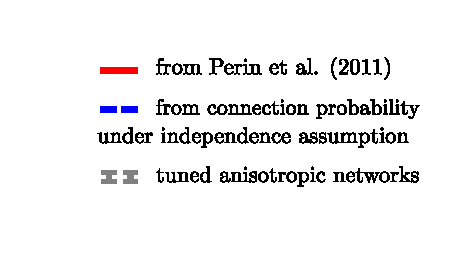
\includegraphics[width=0.5\textwidth]{%
      img/tuned_legend.pdf}   
  }%
  \vspace{-0.15cm}
  \caption{\textbf{Overrepresentation of reciprocal connections
      independent of } Comparison of occurrences of one- and
    bidirectionally connected neuron pairs in (gray) with profiles
    found by \textcite{Perin2011} (red), shows that overrepresentation of
    bidirectional pairs is distance-independent and not connected to
    anisotropy.  \textbf{A)} Overall connection probability in the
    adapted anisotropic networks was successfully tuned to reflect
    connection probability found by Perin et al. \textbf{B)-C)}
    Probabilities for a random neuron pair to display , 
    (\smtcite{875505b0})} %?? fix width issue!!
  \label{fig:perin_profiles_and_such}
\end{figure}


%%% Local Variables: 
%%% mode: latex
%%% TeX-master: "../dplths_document"
%%% End: 
